% !TeX root = ../paper.tex
\hypertarget{method}{%
\section{SmartVLA Framework}\label{method}}

% !TeX root = ../paper.tex
\begin{figure}[H]
  \centering
  \setlength{\parskip}{0pt}
  % Match Figure 1 without negative caption or float spacing.
  \setlength{\abovecaptionskip}{\baselineskip}
  \setlength{\belowcaptionskip}{0pt}
  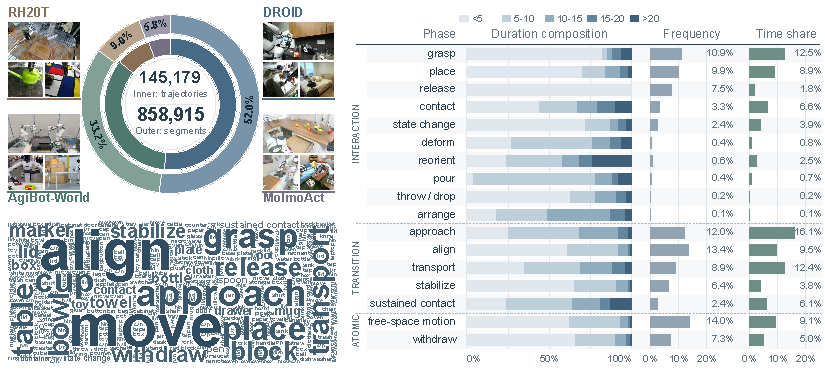
\includegraphics[width=\textwidth,trim=0 4bp 0 0,clip]{figures/fig2_data_construction_from_overleaf_20260924.pdf}\par\nointerlineskip
  \caption{SmartVLA data construction. Left: four trajectory sources,
  aligned segments, and the action vocabulary word cloud. Right:
  subtask duration composition, frequency, and total time across interaction,
  transition, and atomic-motion phases.}
  \label{fig:data-pipeline}
\end{figure}
%

SmartVLA builds on pretrained representations to strengthen instruction-conditioned control while
retaining complete-task execution. Our diagnostics suggest a starting point: target information
remains readable but does not reliably guide actions. Task-level supervision leaves this
correspondence underspecified. For example, ``put the bowl on the plate'' labels approaching,
grasping, transporting, and releasing without specifying the scope of ``approach the bowl'' alone. A
policy may therefore use language as a task identifier and reproduce familiar actions from scene and
execution cues. Whole-task paraphrases diversify descriptions without resolving this local
ambiguity.

Our insight is to change the granularity of supervision--action correspondence: each command should
describe a control phase, with visual prompts specifying its current object or target. Existing
action changes, gripper events, and visual interactions provide evidence for these phases.
Establishing behavioral scope before generating instructions turns open-ended video annotation into
constrained local supervision, reducing reliance on expensive end-to-end video interpretation and
per-segment manual rewriting.

Aligned data alone do not ensure that language influences action selection when visual correlations
can predict familiar behavior. We therefore first learn instruction--motion correspondence without
images, then ground it in observed scenes, and finally adapt to target domains while retaining
complete-task supervision. The data pipeline specifies what behavior a command governs; staged
training encourages the policy to use that correspondence.

\hypertarget{steering-oriented-data-construction}{%
\subsection{Action-Aligned Data Construction Pipeline}\label{steering-oriented-data-construction}}

We represent local supervision as $r_i=(\mathbf O_i,\mathbf S_i,\mathbf A_i,c_i,z_i,g_i)$:
observations, robot states, and actions span a segment of length $L_i$, while $c_i$, $z_i$, and
$g_i$ denote its instruction, object/target evidence, and interaction grade.
Figure~\ref{fig:overview}(b) summarizes the pipeline.

\textbf{Establish behavioral scope.} Uniform cuts may split a grasp or combine distinct control
phases. We instead identify boundaries from action changes, gripper events, and visual interactions,
consolidate them using temporal consistency and task-family rules, and associate each segment with
object and target evidence. This evidence constrains what the subsequent instruction should
describe. The aim is not simply to shorten trajectories, but to align the instruction's execution
scope with control-phase boundaries, reducing the inclusion of subsequent actions outside the
current requirement.

\textbf{Match rewrites to interaction evidence.} We use three families: \textbf{Object-free atomic
motion} specifies movement without object names; \textbf{Synonym/task rewrite} varies wording while
preserving the local goal; and \textbf{Spatial visual generalization} pairs instructions with
points, boxes, regions, or trajectories rendered in the observations. Low, Mid, and High grades
correspond to free-space motion, transitions, and explicit object interaction. Low excludes spatial
rewrites without supported targets; High excludes atomic rewrites that omit essential object
relations; Mid permits all three (Table~\ref{tab:grade-policies}). For example, free-space motion
such as ``move up'' need not identify an object, whereas placement must preserve what is placed and
where. Grades therefore govern rewrite applicability and specificity, not segment retention.

\begingroup
% The preceding paragraph already separates this block from the text above.
% Avoid adding wrapfig's extra top inset; keep caption-to-table spacing below.
\setlength{\intextsep}{0pt}
% !TeX root = ../paper.tex
\begin{wraptable}[10]{r}{0.38\textwidth}
\centering
\normalsize
% Keep one body-line gap between the caption and the table.
\setlength{\parskip}{0pt}
\setlength{\abovecaptionskip}{0pt}
\setlength{\belowcaptionskip}{\baselineskip}
\caption{\centering Grade-conditioned rewrite families.}
\label{tab:grade-policies}
\nointerlineskip
\setlength{\tabcolsep}{2.0pt}
\begin{tabular}{@{}lccc@{}}
\toprule
Grade & \shortstack{Atomic\\motion} & \shortstack{Synonym/\\task} & \shortstack{Spatial\\visual} \\
\midrule
Low & yes & yes & no \\
Mid & yes & yes & yes \\
High & no & yes & yes \\
\bottomrule
\end{tabular}
\end{wraptable}
%

\textbf{Generate and review.} The generator receives the phase, grade, and available evidence, while
automated semantic and visual review filters inconsistent rewrites. Separating evidence extraction,
constrained generation, and review supports scalable construction without requiring the language
model to infer the entire temporal structure. Local examples form $\mathcal D_{\mathrm{local}}$;
examples retaining original task instructions form $\mathcal D_{\mathrm{task}}$, preserving
supervision of complete execution. Figure~\ref{fig:data-pipeline} summarizes the corpus.
Appendix~\ref{appendix:data-construction} provides implementation details and illustrates the
pipeline and segment-level examples in Figure~\ref{fig:appendix-action-aligned-pipeline}.

\par
\endgroup

\hypertarget{steering-centric-policy-training}{%
\subsection{Three-Stage Training Recipe}\label{steering-centric-policy-training}}

We separate learning how instructions specify motion, how observations locate its target, and how
both transfer to a target domain (Figure~\ref{fig:overview}(c)). Let $\theta=(\psi,\phi)$ collect
the backbone and action-head parameters. The policy predicts $\mathbf A_t=\mathbf
a_{t:t+H-1}\sim\pi_\theta(\cdot\mid\mathbf o_t,\mathbf s_t,c_t)$; prediction length $H$ is distinct
from segment length $L_i$. All stages retain the native per-example action loss
$\ell_{\mathrm{act}}$, with objective
\begin{equation}
\label{eq:action-objective}
\mathcal L_{\mathrm{act}}(\theta;\mathcal D)=
\mathbb E_{(\mathbf o,\mathbf s,c,\mathbf A)\sim\mathcal D}
\left[\ell_{\mathrm{act}}(\theta;\mathbf o,\mathbf s,c,\mathbf A)\right].
\end{equation}

\textbf{Warmup: learn motion correspondence without image-based shortcuts.} Atomic instructions
specify motion without requiring object localization. Warmup therefore receives only atomic
instructions and robot state, freezes the backbone at $\psi_0$, and trains the action head with
$\mathcal L_{\mathrm w}(\phi)=\mathcal L_{\mathrm{act}}((\psi_0,\phi);\mathcal
D_{\mathrm{atomic}})$. Here $\mathcal D_{\mathrm{atomic}}$ contains eligible Low/Mid segments with
no image input. Different atomic commands specify corresponding motion patterns, while robot state
supplies the physical conditions for execution. Removing images prevents initial learning from
directly relying on visual scene cues; freezing the backbone focuses optimization on how the action
head uses existing representations, establishing a language-conditioned action prior for subsequent
visually conditioned learning.

\textbf{Pretraining: ground the prior in current scenes.} Motion alone does not identify its target:
``lift the object in the red box'' also requires binding the prompt to the current object. Starting
from warmup, we restore multi-view images and train both modules with $\mathcal L_{\mathrm
p}(\theta)=\mathcal L_{\mathrm{act}}(\theta;\mathcal D_{\mathrm{mix}}^{\mathrm{pre}})$. The mixture
$\mathcal D_{\mathrm{mix}}=\alpha\mathcal D_{\mathrm{task}}+(1-\alpha)\mathcal D_{\mathrm{local}}$
samples original-task and local supervision, respectively. Local commands and visual prompts teach
scene-dependent control, while original-task examples retain complete-task supervision. The
resulting checkpoint is SmartVLA-Base.

\textbf{Adaptation: retain both supervision granularities.} Original-task instructions alone do not
preserve local command--action supervision, while local segments cannot replace supervision of
complete execution. We therefore reconstruct target-domain demonstrations using
Section~\ref{steering-oriented-data-construction} and independently adapt each domain $d$ from
SmartVLA-Base, optimizing both modules with $\mathcal L_{\mathrm a}^{d}(\theta)=\mathcal
L_{\mathrm{act}}(\theta;\mathcal D_{\mathrm{mix}}^{d})$. This continues local language and visual
supervision while learning target-domain control.

SmartVLA-Pi and SmartVLA-OFT follow this recipe with their native action models. Both accept
complete-task, subtask, or updated corrective commands through the same observation-conditioned
interface. Architectures, initialization, sampling ratios, training settings, and the calling
protocol are detailed in Appendix~\ref{appendix:model-details}.

